\documentclass[finnish,english,t]{beamer}
%\documentclass[finnish,english,handout]{beamer}

% Uncomment if want to show notes
% \setbeameroption{show notes}

\mode<presentation>
{
  \usetheme{Copenhagen}
  % oder ...

  %\setbeamercovered{transparent}
  % oder auch nicht
}


% \usepackage[pdftex]{graphicx}
\usepackage[T1]{fontenc}
\usepackage[latin1]{inputenc}
\usepackage{times}
\usepackage{epic,epsfig}
\usepackage{subfigure,float}
\usepackage{amsmath,amsfonts,amssymb}
\usepackage{inputenc}
\usepackage{babel}
\usepackage{afterpage}
\usepackage{url}
\urlstyle{same}
\usepackage{eufrak}
\usepackage{amsbsy}
\usepackage{eucal}
\usepackage{rotating}
\usepackage[all,poly,ps,color]{xy}

\usepackage{natbib}
\bibliographystyle{apalike}

% \definecolor{hutblue}{rgb}{0,0.2549,0.6784}
% \definecolor{midnightblue}{rgb}{0.0977,0.0977,0.4375}
% \definecolor{hutsilver}{rgb}{0.4863,0.4784,0.4784}
% \definecolor{lightgray}{rgb}{0.95,0.95,0.95}
% \definecolor{section}{rgb}{0,0.2549,0.6784}
% \definecolor{list1}{rgb}{0,0.2549,0.6784}
 \definecolor{navyblue}{rgb}{0,0,0.5}
\renewcommand{\emph}[1]{\textcolor{navyblue}{#1}}

\graphicspath{{./figs/}}

\pdfinfo{
  /Title      (Bayesian data analysis, ch 10)
  /Author     (Aki Vehtari) %
  /Keywords   (Bayesian probability theory, Bayesian inference, Bayesian data analysis)
}


\parindent=0pt
\parskip=8pt
\tolerance=9000
\abovedisplayshortskip=0pt

\setbeamertemplate{navigation symbols}{}
\setbeamertemplate{headline}[default]{}
\setbeamertemplate{headline}[text line]{\insertsection}
\setbeamertemplate{footline}[frame number]


\def\o{{\mathbf o}}
\def\t{{\mathbf \theta}}
\def\w{{\mathbf w}}
\def\x{{\mathbf x}}
\def\y{{\mathbf y}}
\def\z{{\mathbf z}}

\DeclareMathOperator{\E}{E}
\DeclareMathOperator{\Var}{Var}
\DeclareMathOperator{\var}{var}
\DeclareMathOperator{\Sd}{Sd}
\DeclareMathOperator{\sd}{sd}
\DeclareMathOperator{\Gammad}{Gamma}
\DeclareMathOperator{\Invgamma}{Inv-gamma}
\DeclareMathOperator{\Bin}{Bin}
\DeclareMathOperator{\Negbin}{Neg-bin}
\DeclareMathOperator{\Poisson}{Poisson}
\DeclareMathOperator{\Beta}{Beta}
\DeclareMathOperator{\logit}{logit}
\DeclareMathOperator{\N}{N}
\DeclareMathOperator{\U}{U}
\DeclareMathOperator{\BF}{BF}
\DeclareMathOperator{\Invchi2}{Inv-\chi^2}
\DeclareMathOperator{\NInvchi2}{N-Inv-\chi^2}
\DeclareMathOperator{\InvWishart}{Inv-Wishart}
\DeclareMathOperator{\tr}{tr}
% \DeclareMathOperator{\Pr}{Pr}
\def\euro{{\footnotesize \EUR\, }}
\DeclareMathOperator{\rep}{\mathrm{rep}}

\title[]{Bayesian data analysis}
\subtitle{}

\author{Aki Vehtari}

\institute[Aalto]{}

\begin{document}

\begin{frame}
  
  {\Large\color{navyblue} Chapter 10}

  \begin{itemize}
\item 10.1 Numerical integration (overview)
\item 10.2 Distributional approximations (overview, more in Chapter 4 and 13)
\item 10.3 Direct simulation and rejection sampling (overview)
\item 10.4 Importance sampling (used in PSIS-LOO discussed later)
\item 10.5 How many simulation draws are needed? (Ex 10.1 and 10.2)
\item 10.6 Software (can be skipped)
\item 10.7 Debugging (can be skipped)
   \end{itemize}
\end{frame}

\begin{frame}
  
  {\Large\color{navyblue} Notation}

  \begin{itemize}
  \item In this chapter, generic $p(\theta)$ is used instead of
    $p(\theta|y)$
  \item unnormalized distribution is denoted by $q(\cdot)$
  \item proposal distribution is denoted by $g(\cdot)$
  \end{itemize}

\end{frame}

\begin{frame}
  
  {\Large\color{navyblue} Numerical accuracy}

  \begin{itemize}
  \item Floating point presentation of numbers. e.g. with 64bits
    \begin{itemize}
    \item closest value to zero is $\approx 2.2\cdot 10^{-308}$
      \begin{itemize}
      \item qr=rnorm(600);prod(dnorm(qr)) $\rightarrow$ 0
      \item<3-> pbeta(0.5,241945,251527, lower.tail=FALSE) $\approx -1.15\cdot 10^{-42}$
      \end{itemize}
    \item<2-> closest value to 1 is $\approx 1 \pm  2.2\cdot 10^{-16}$
      \begin{itemize}
      \item pbeta(0.5,241945,251527) $\rightarrow$ 1
      \end{itemize}
    \end{itemize}
  \item<4-> Log densities
    \begin{itemize}
    \item use log densities to avoid over- and underflows in floating
      point presentation
      \begin{itemize}
      \item sum(dnorm(qr,log=TRUE)) $\rightarrow$ -847.3
      \item<5-> how many observations we can now handle? % $\sim 10^308$
    \end{itemize}
    \item<6-> compute exp as late as possible
      \begin{itemize}
      \item e.g. for $a>b$, compute $\log(\exp(a)+\exp(b)) = a + \log(1+\exp(b-a))$\\
        e.g. $\log(exp(800)+exp(800)) \rightarrow$ Inf, but $800 + \log(1 + exp(800-800)) \approx 800.69$
      \item<7-> e.g. in Metropolis-algorithm compute the log of ratio of densities using the identity\\
        $\log(a/b)=\log(a)-\log(b)$
    \end{itemize}
    \end{itemize}
  \end{itemize}

\end{frame}


 \begin{frame}
   
  {\Large\color{navyblue} It's all about expectations}

   \begin{align*}
   E_{\theta}[f(\theta)] = \int f(\theta) p(\theta|y) d\theta
   \end{align*}

  \begin{itemize}
  \item Conjugate priors and analytic solutions
  \item Grid integration and other quadrature rules
  \item Independent Monte Carlo, rejection and importance sampling
  \item Markov Chain Monte Carlo
  \item Distributional approximations (Laplace, VB, EP)
  \end{itemize}
   

 \end{frame}


\begin{frame}
   
  {\Large\color{navyblue} Quadrature integration}

  \begin{itemize}
  \item The simplest quadrature integration is grid integration
    \begin{itemize}
    \item Evaluate function in a grid and compute
    \begin{minipage}{4cm}
    \begin{align*}
      \E[-\alpha/\beta] \approx \sum_{t=1}^{T} w_{\mathrm{cell}}^{(t)} \frac{\alpha^{(t)}}{\beta^{(t)}},
    \end{align*}
  \end{minipage}
  \begin{minipage}{5cm}
  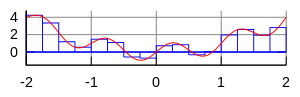
\includegraphics[width=5cm]{Integration_rectangle.png}
\end{minipage}
where $w_{\mathrm{cell}}^{(t)}$ is the normalized probability of a grid cell $t$, and $\alpha^{(t)}$ and $\beta^{(t)}$ are center locations of grid cells
\end{itemize}
\item<2-> In 1D further variations, e.g. trapezoid
  \begin{center}
    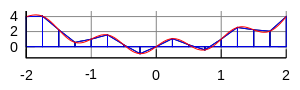
\includegraphics[width=5cm]{Integration_trapezoid.png}
  \end{center}
\item<3-> In 2D and higher
  \begin{itemize}
  \item nested quadrature
  \item product rules
  \end{itemize}
  \end{itemize}
  

\end{frame}


\begin{frame}
  
  {\Large\color{navyblue} Monte Carlo - history}

  \begin{itemize}
  \item Used already before computers
    \begin{itemize}
      \item Buffon (18th century; needles)
      \item De Forest, Darwin, Galton (19th century)
      \item Pearson (19th century; roulette)
      \item Gosset (Student, 1908; hat)
    \end{itemize}
    \pause
  \item "Monte Carlo method" term was proposed by Metropolis, von Neumann
    or Ulam in the end of 1940s
     \begin{itemize}
     \item they worked together in atomic bomb project
     \item Metropolis and Ulam, "The Monte Carlo Method", 1949
     \end{itemize}
    \pause
   \item Bayesians started to have enough cheap computation time in 1990s
     \begin{itemize}
     \item BUGS project started 1989 (last OpenBUGS release 2014)
     \item Gelfand \& Smith, 1990
     \item Stan initial release 2012
     \end{itemize}
     % \begin{itemize}
     %   \item t�t� ennen k�ytt� v�h�ist�, vaikka bayesilaisiakin
     %     osallistui teorian ja menetelmien kehitt�miseen
     % \end{itemize}
  \end{itemize}

\end{frame}

% \note{Buffon tiputteli neuloja lautalattialle
% % http://noppa5.pc.helsinki.fi/koe/flash/prob/buf-en.html

% Pearson laski kuinka monta ruletinpy�rityst� tarvitaan,
% t�t� tietoa joku muu hy�dynsikin

% Gosset k�ytti paperilappuja

% atomipommin kehitt�jill� oli laskentatehoa

% }

\begin{frame}
  
  {\Large\color{navyblue} Monte Carlo}

  \begin{itemize}
  \item Simulate samples from the target distribution
    \begin{itemize}
    \item these samples can be treated as any observations
    \end{itemize}
  \item Use these samples, for example,
    \begin{itemize}
    \item to compute means, deviations, quantiles
    \item to draw histograms
    \item to marginalize
    \item etc.
    \end{itemize}
  \end{itemize}

\end{frame}

\begin{frame}

  
  {\Large\color{navyblue} Monte Carlo vs. deterministic}

  \begin{itemize}
  \item Monte Carlo = simulation methods
    \begin{itemize}
    \item evaluation points are selected stochastically (randomly)
    \end{itemize}
  \item Deterministic methods (e.g. grid)
    \begin{itemize}
    \item evaluation points are selected by some deterministic rule
    \end{itemize}
  \end{itemize}

\end{frame}

\begin{frame}

  
  {\Large\color{navyblue} How many simulation samples are needed?}

  \begin{itemize}
  \item If samples are independent
    \begin{itemize}
    \item usual methods to estimate the uncertainty due to a finite
      number of observations
    \end{itemize}
  \item Markov chain Monte Carlo produces dependent samples
    \begin{itemize}
    \item requires additional work to estimate the \emph{effective
        number of samples}
    \end{itemize}
  \end{itemize}

\end{frame}

\begin{frame}
  
  {\Large\color{navyblue} How many simulation samples are needed?}

  \begin{itemize}
  \item Expectation of unknown quantity
    \begin{equation*}
      \E(\theta)\approx \frac{1}{L}\sum_l \theta^{(l)}
    \end{equation*}
    if $L$ is big and $\theta^{(l)}$ are independent, way may assume
    that the distribution of the expectation approaches normal
    distribution (see Ch 4) with variance $\sigma^2_\theta/L$
    (asymptotic normality)
    \begin{itemize}
    \item this variance is independent on dimensionality of $\theta$
      \pause
    \item total variance is sum of the epistemic unecrtainty in the
      posterior and the uncertainty due to using finite number of
      Monte Carlo samples
      \begin{equation*}
        \sigma^2_\theta+\sigma^2_\theta/L \pause= \sigma^2_\theta(1+1/L)
      \end{equation*}
      \pause
      \vspace{-5mm}
    \item e.g. if $L=100$, deviation increases by $\sqrt{1+1/L}=1.005$\\
      ie. Monte Carlo error is very small (for the expectation)
      \pause
    \item See Ch 4 for counter-examples for asymptotic normality
    \end{itemize}
\end{itemize}

\end{frame}

\begin{frame}
  
  {\Large\color{navyblue} Example: Kilpisj�rvi summer temperature}

  Average temperature in June, July, and August at Kilpisj�rvi, Finland

  \begin{center}
    \only<1>{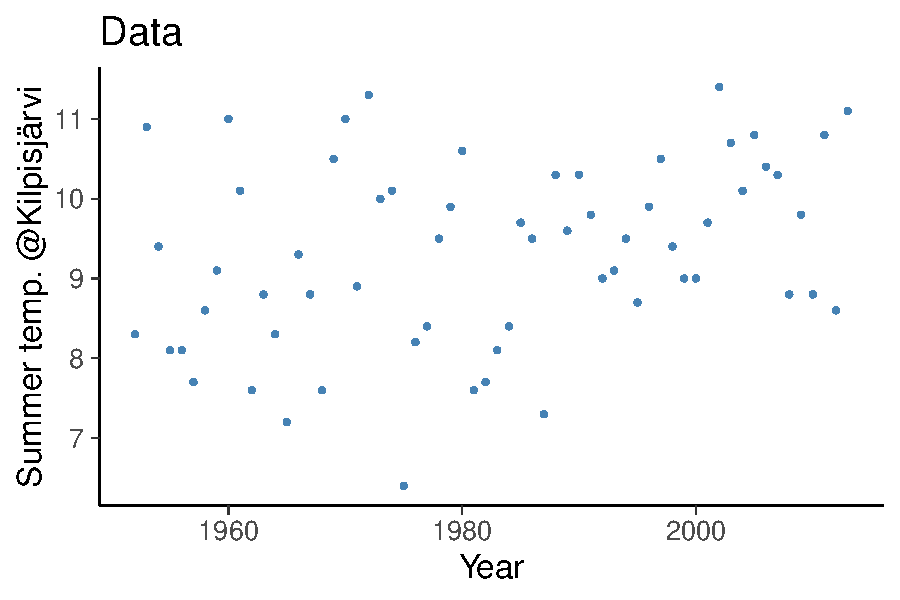
\includegraphics[width=8cm]{kilpis_data.pdf}}
    \only<2>{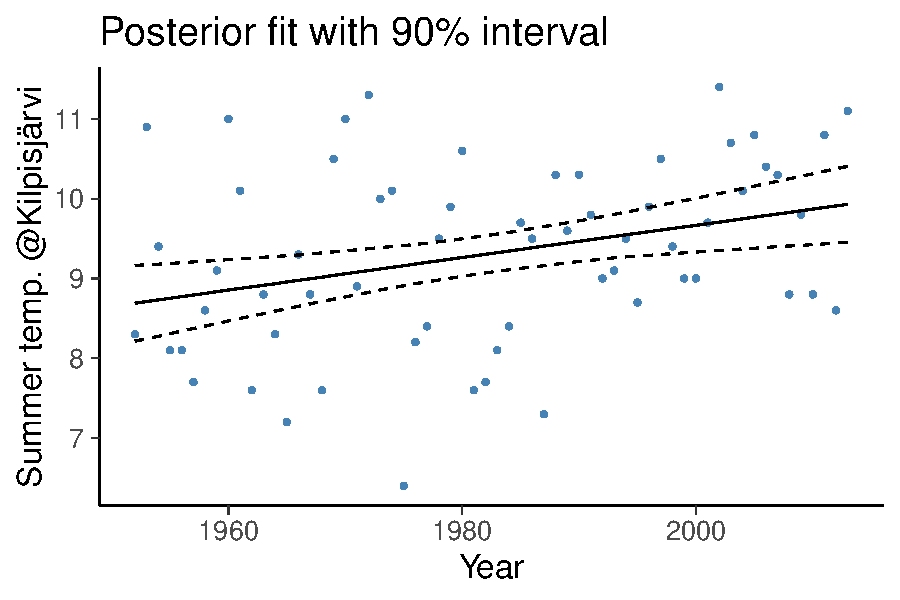
\includegraphics[width=8cm]{kilpis_pfit.pdf}}
  \end{center}

\end{frame}

\begin{frame}
  
  {\Large\color{navyblue} Example: Kilpisj�rvi summer temperature}

  \begin{center}
    \only<1>{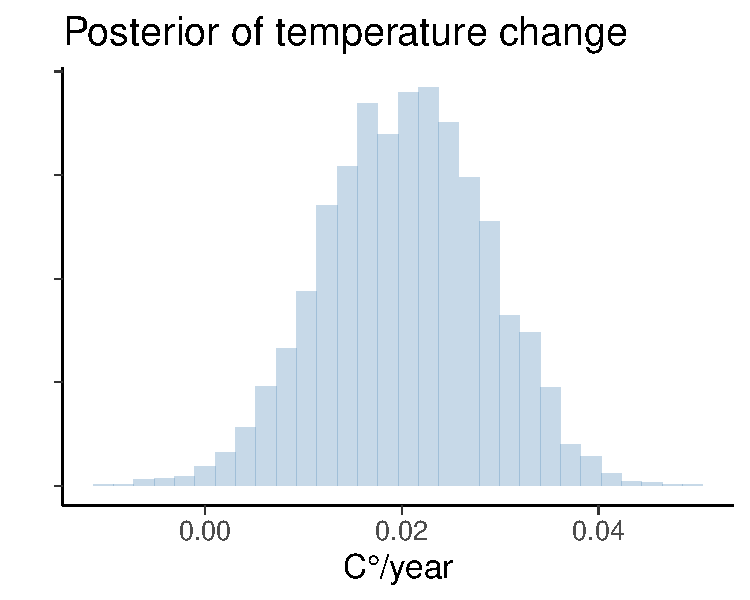
\includegraphics[width=8cm]{kilpis_phist.pdf}}
    \only<2>{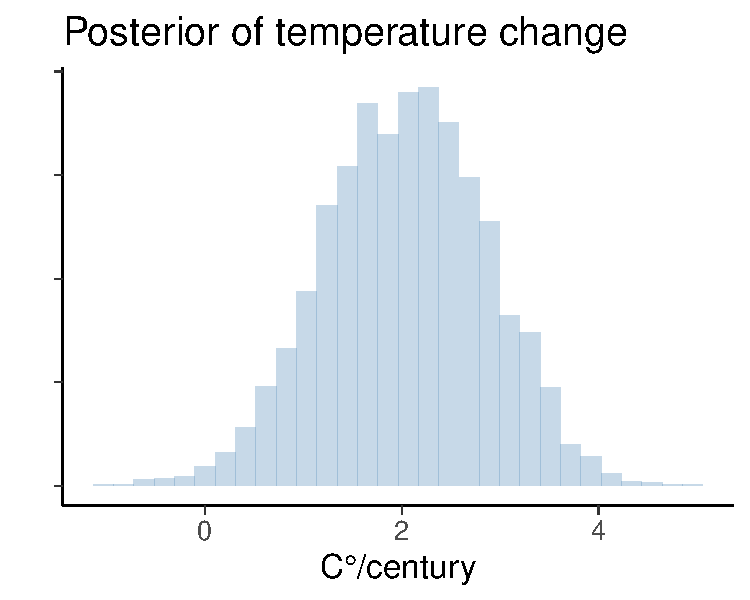
\includegraphics[width=8cm]{kilpis_phist100.pdf}}
    \only<3>{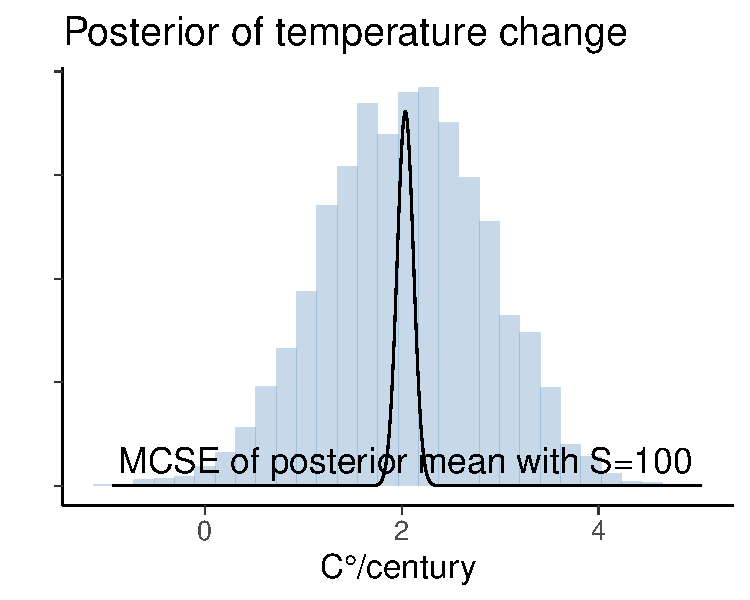
\includegraphics[width=8cm]{kilpis_phist100_mcse1a.pdf}}
    \only<4>{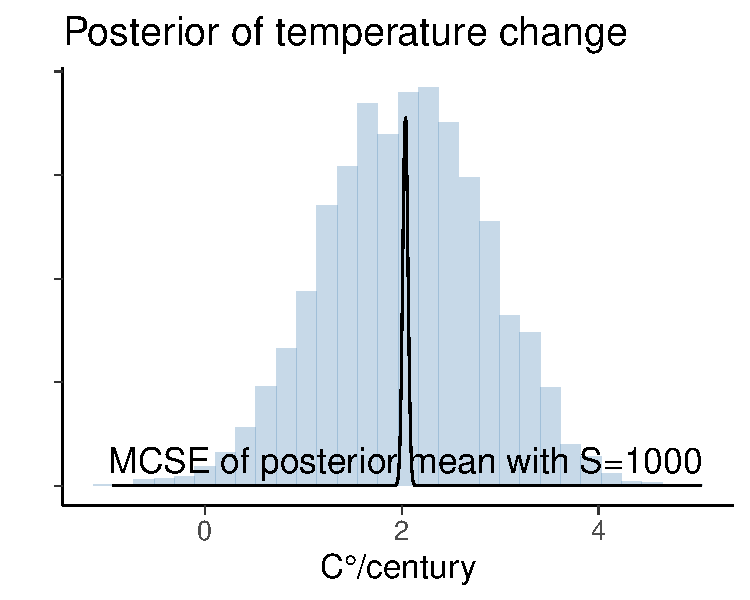
\includegraphics[width=8cm]{kilpis_phist100_mcse1b.pdf}}
    \only<3>{$\sigma_\theta\approx 0.827,\, \text{MCSE} \approx 0.0827,\, \text{total deviation} \approx 0.831$}
    \only<4>{$\sigma_\theta\approx 0.827,\, \text{MCSE} \approx 0.0261,\, \text{total deviation} \approx 0.827$}
  \end{center}

\end{frame}

\begin{frame}
  
  {\Large\color{navyblue} Example: Kilpisj�rvi summer temperature}

  \vspace{\baselineskip}
  \makebox[12cm][t]{
    \hspace{-0.9cm}
  \begin{minipage}[b][12cm][t]{12cm}
    \only<1->{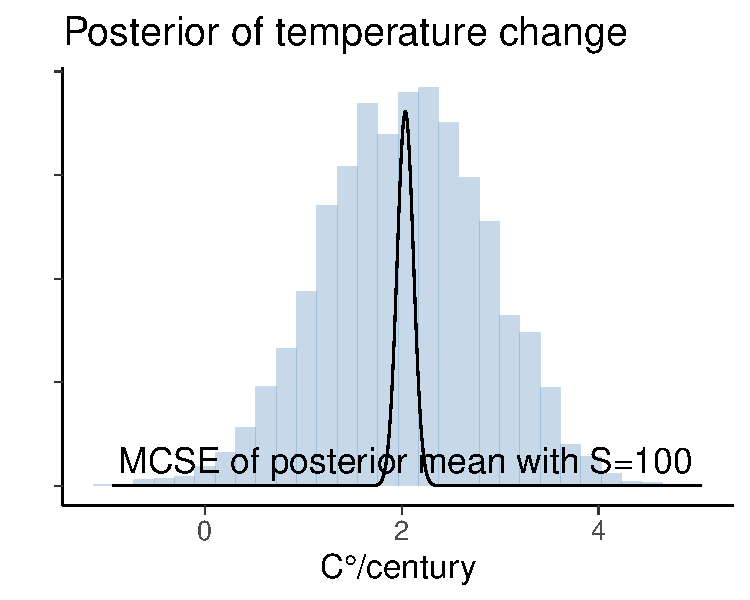
\includegraphics[width=4cm]{kilpis_phist100_mcse1a.pdf}}
    \only<2->{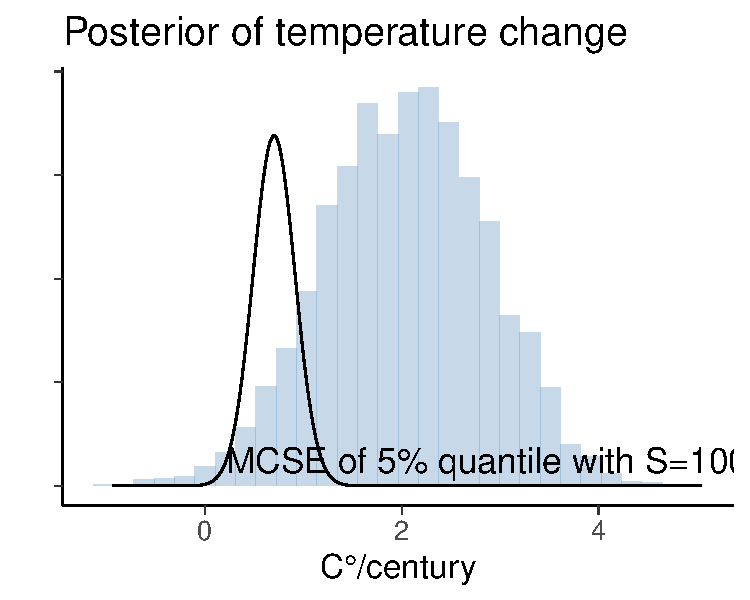
\includegraphics[width=4cm]{kilpis_phist100_mcse2a.pdf}}
    \only<3->{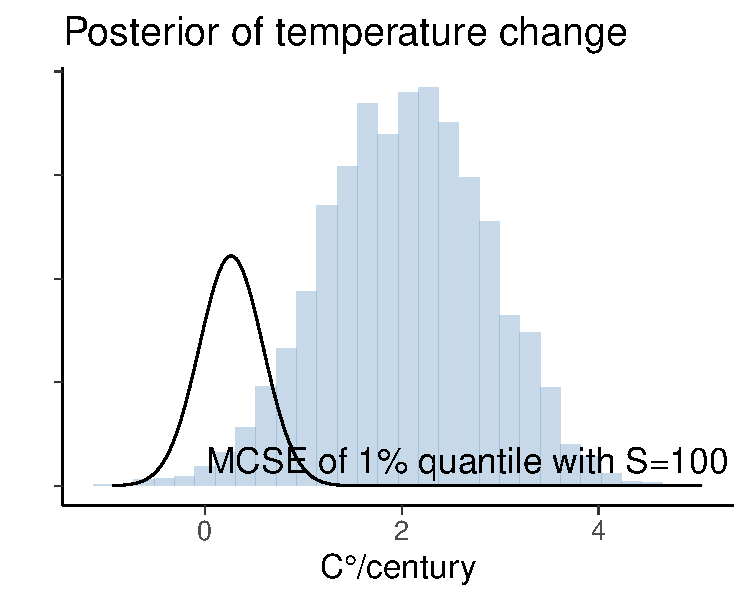
\includegraphics[width=4cm]{kilpis_phist100_mcse3a.pdf}}\\
    \only<1->{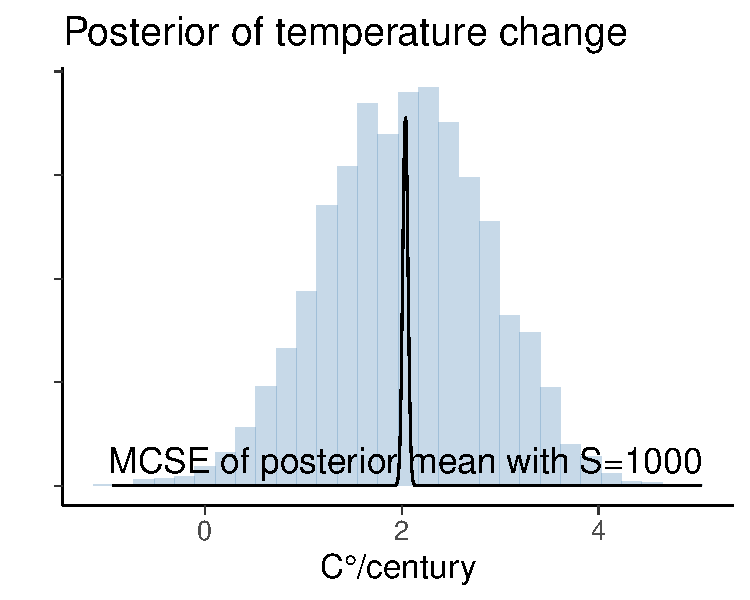
\includegraphics[width=4cm]{kilpis_phist100_mcse1b.pdf}}
    \only<2->{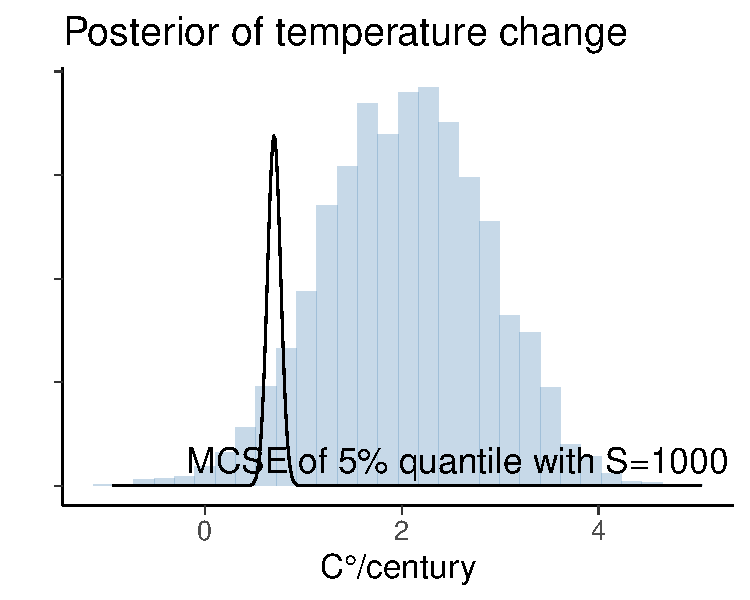
\includegraphics[width=4cm]{kilpis_phist100_mcse2b.pdf}}
    \only<3->{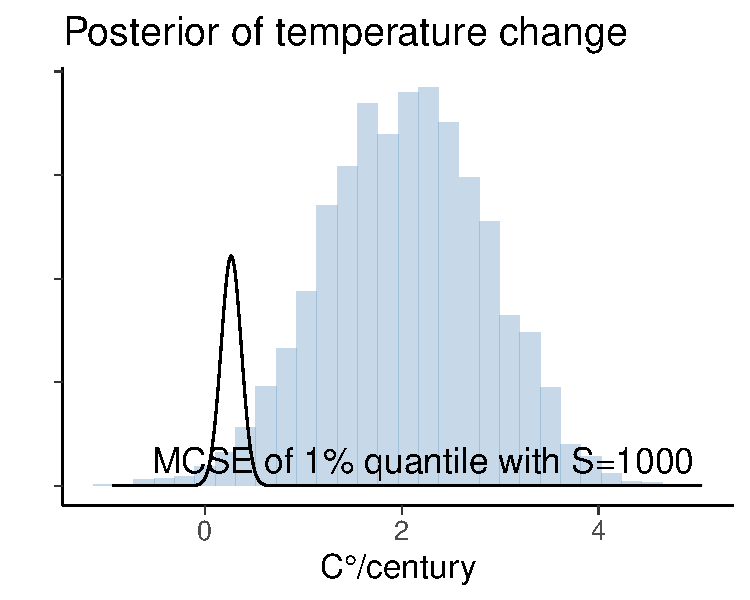
\includegraphics[width=4cm]{kilpis_phist100_mcse3b.pdf}}\\
    \begin{center}
      \vspace{-\baselineskip}
  \only<4->{Tail quantiles are more difficult to estimate}
\end{center}
  \end{minipage}
  }

\end{frame}

\begin{frame}
  
  {\Large\color{navyblue} How many simulation samples are needed?}

  \begin{itemize}
  \item Posterior probability
    \begin{equation*}
      p(\theta \in A)\approx \frac{1}{L}\sum_l I(\theta^{(l)} \in A)
    \end{equation*}
    where $I(\theta^{(l)} \in A)=1$ if $\theta^{(l)} \in A$
    \begin{itemize}
    \item $I(\cdot)$ is binomially distributed as $p(\theta \in A)$
        \begin{itemize}
        \item[$\rightarrow$] $\var(I(\cdot)) =  p(1-p)$  (Appendix A, p. 579)
        \item[$\rightarrow$] standard deviation of $p$ is $\sqrt{p(1-p)/L}$
        \end{itemize}
        \pause
      \item if $L=100$ and $p\approx 0.5$, $\sqrt{p(1-p)/L}=0.05$\\
        ie. accuracy is about $5\%$ units
        \pause
      \item $L=2500$ simulation samples needed for $1\%$ unit accuracy
    \end{itemize}
    \pause
  \item To  estimate small probabilities, a large number of samples is needed
    \begin{itemize}
    \item to be able to estimate $p$, need to get samples with
      $\theta^{(l)} \in A$, which in expectation requires $L \gg 1/p$
    \end{itemize}
\end{itemize}

\end{frame}

\begin{frame}
  
  {\Large\color{navyblue} Example: Kilpisj�rvi summer temperature}

  \begin{center}
    \only<1>{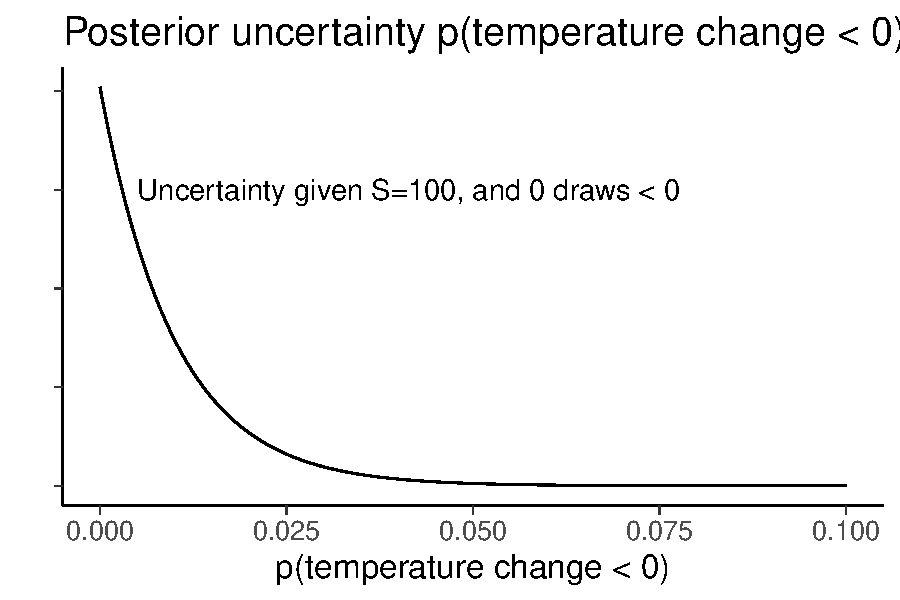
\includegraphics[width=10cm]{kilpis_ppneg_mcse1a.pdf}}
    \only<2>{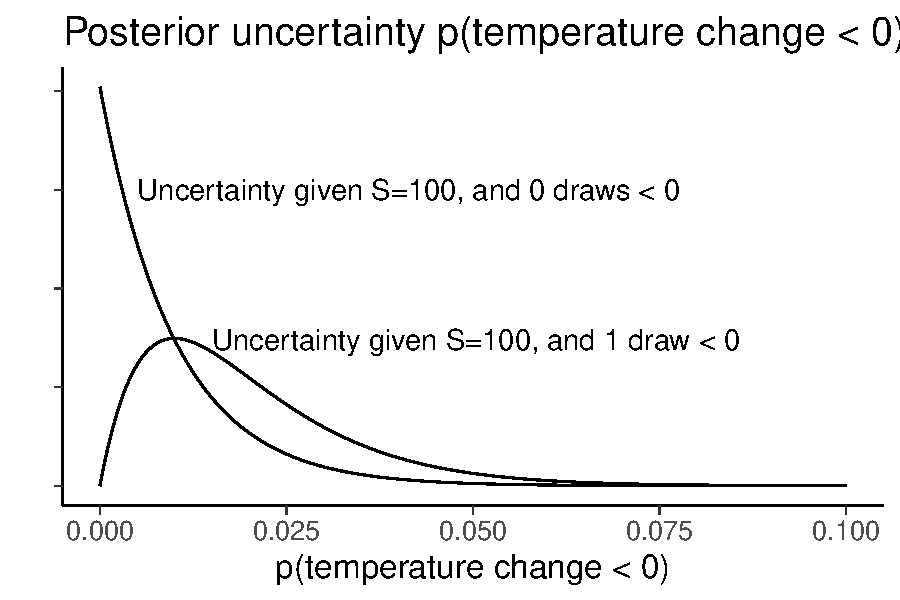
\includegraphics[width=10cm]{kilpis_ppneg_mcse1b.pdf}}
    \only<3>{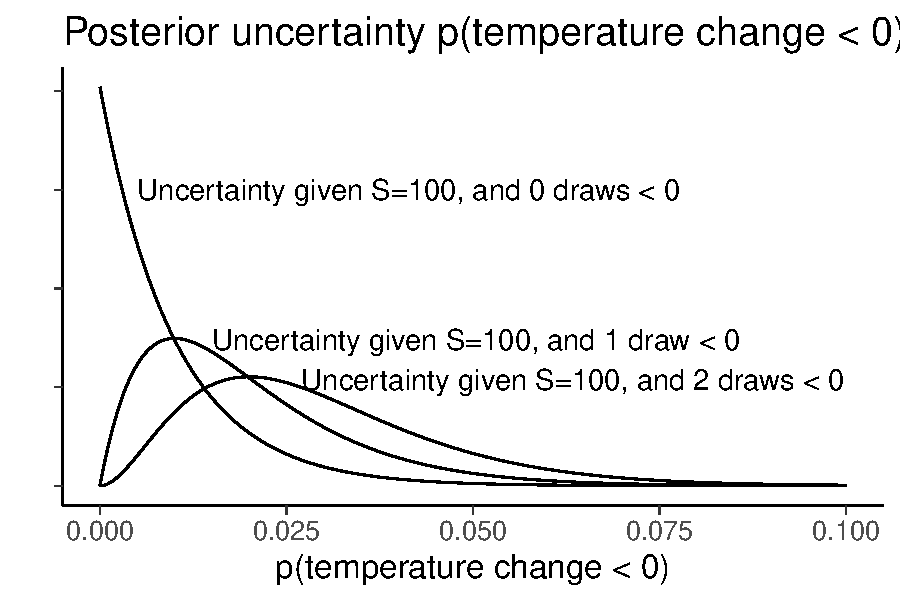
\includegraphics[width=10cm]{kilpis_ppneg_mcse1c.pdf}}
    \only<4>{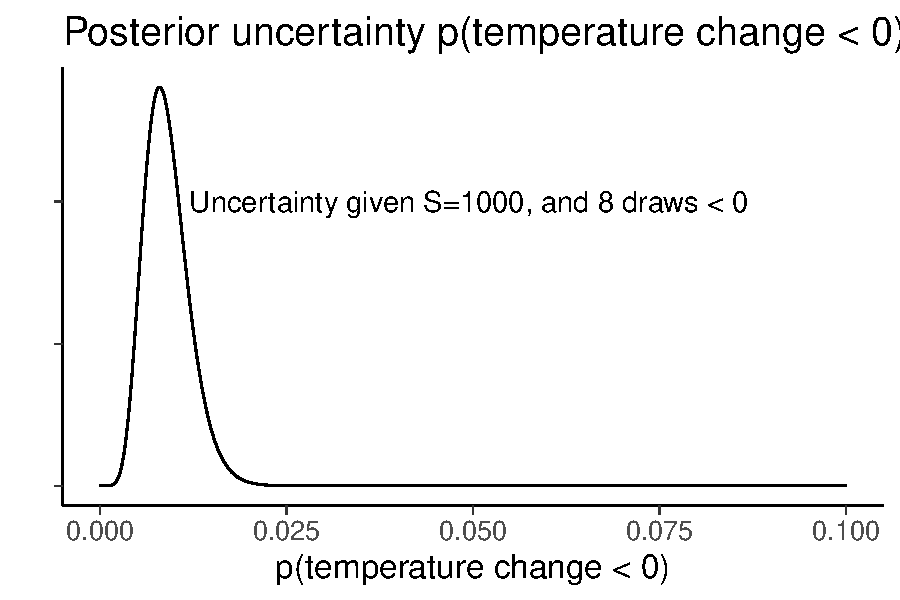
\includegraphics[width=10cm]{kilpis_ppneg_mcse1000.pdf}}
    \only<5>{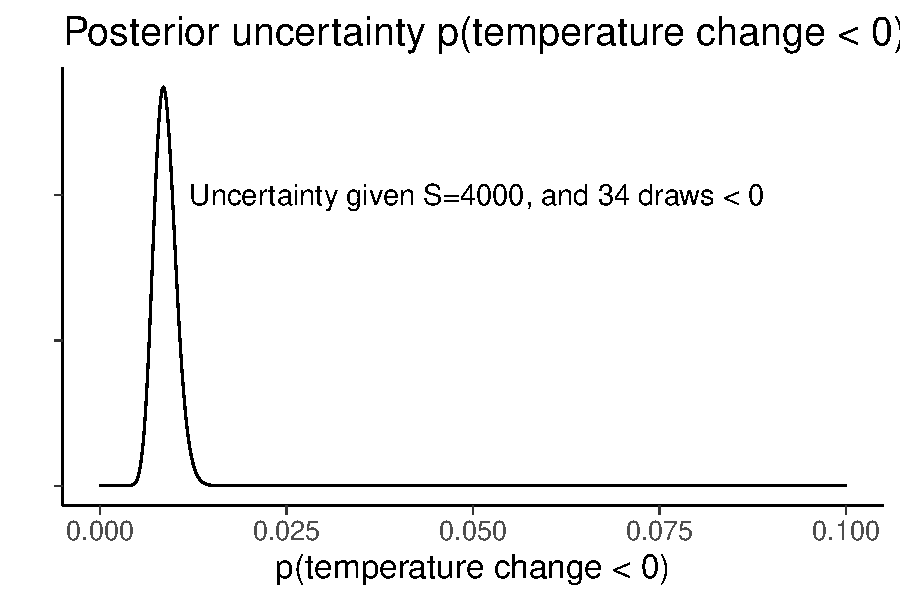
\includegraphics[width=10cm]{kilpis_ppneg_mcse4000.pdf}}
  \end{center}

\end{frame}

\begin{frame}
  
  {\Large\color{navyblue} How many simulation samples are needed?}

  \begin{itemize}
  \item Less samples needed with
    \begin{itemize}
    \item deterministic methods
    \item marginalization (Rao-Blackwellization)
    \item variance reduction methods, such, control variates
    \end{itemize}
  \end{itemize}

\end{frame}

\begin{frame}
  
  {\Large\color{navyblue} How many simulation samples are needed?}

  \begin{itemize}
  \item Number of independent samples needed doesn't depend on the number of dimensions
    \begin{itemize}
    \item but it may be difficult to obtain independent samples in high dimensional case
    \end{itemize}
  \end{itemize}

\end{frame}

\begin{frame}

  
  {\Large\color{navyblue} Direct simulation}

  \begin{itemize}
  \item Produces independent samples
    \begin{itemize}
    \item Using analytic transformations of unifrom random numbers
      (eg. appendix A)
    \item factorization
    \item numerical inverse-cdf
    \end{itemize}
  \item Problem: restricted to limited set of models
  \end{itemize}

\end{frame}

\begin{frame}

  {\Large\color{navyblue} Random number generators}

  \begin{itemize}
  \item Good pseudo random number generators are sufficient for
    Bayesian inference
    \begin{itemize}
    \item pseudo random generator uses deterministic algorithm to
      produce a sequence which is difficult to make difference from
      truly random sequence
    \item modern software used for statistical analysis have good
      pseudo RNGs
    \end{itemize}
  \end{itemize}

\end{frame}

\begin{frame}

  
  {\Large\color{navyblue} Direct simulation: Example}

  \begin{itemize}
  \item Box-Muller -method:\\ If $U_1$ and $U_2$ are independent
    draws from distribution $\U(0,1)$, and
    \begin{align*}
      X_1 & = \sqrt{-2\log(U_1)}\cos(2\pi U_2) \\
      X_2 & = \sqrt{-2\log(U_1)}\sin(2\pi U_2)
    \end{align*}
    then $X_1$ and $X_2$ are independent samples from the distribution
    $\N(0,1)$
    \pause
    \begin{itemize}
      \item not the fastest method due to trigonometric computations
      \item for normal distrbution more than ten different methods
      \item e.g. R uses inverse-CDF
    \end{itemize}
  \end{itemize}

\end{frame}

\begin{frame}
  
  {\Large\color{navyblue} Grid sampling and curse of dimensionality}

  \begin{itemize}
      \item 10 parameters
      \item if we don't know beforehand where the posterior mass is
        \begin{itemize}
          \item need to choose wide box for the grid
          \item need to have enough grid points to get some of them
            where essential mass is
        \end{itemize}
      \item e.g. 50 or 1000 grid points per dimension
        \begin{itemize}
        \item[$\rightarrow$] 50$^{10} \approx$ 1e17 grid points
        \item[$\rightarrow$] 1000$^{10} \approx$ 1e30 grid points
        \end{itemize}
      \item R and my current laptop can compute density of normal
        distribution about 20 million times per second
        \begin{itemize}
        \item[$\rightarrow$] evaluation in 1e17 grid points would take
           150 years %triljoona vuotta
        \item[$\rightarrow$] evaluation in 1e30 grid points would take
           1 500 billion years %triljoona vuotta
        \end{itemize}
 \end{itemize}

\end{frame}

\begin{frame}
  
  {\Large\color{navyblue} Indirect sampling}
  
  \begin{itemize}
  \item Rejection sampling
    % \begin{itemize}
    % \item draw directly from a proposal distribution, reject some
    %   draws, remaining draws are independent draws from the target
    %   distribution
    % \end{itemize}
    % \pause
  \item Importance sampling
    % \begin{itemize}
    % \item draw directly from a proposal distribution, weight the draws
    % \end{itemize}
    % \pause
  \item Markov chain Monte Carlo (next week)
    % \begin{itemize}
    % \item draw directly from a transition distribution forming a
    %   Markov chain, draws are dependent draws from the target
    %   distribution
    % \end{itemize}
  \end{itemize}

\end{frame}

\begin{frame}
  
  {\Large\color{navyblue} Rejection sampling}

    \vspace{-.3\baselineskip}
  \begin{itemize}
  \item[-] Proposal forms envelope over the target distribution ${q(\theta|y)}/{M g(\theta)} \leq 1$
  \item[-] Draw from the proposal and accept with probability ${M g(\theta)}/{q(\theta|y)}$
  \item<3>[-] Common for truncated distributions
  \end{itemize}
  \begin{center}
    \vspace{-1.6\baselineskip}
    \only<1>{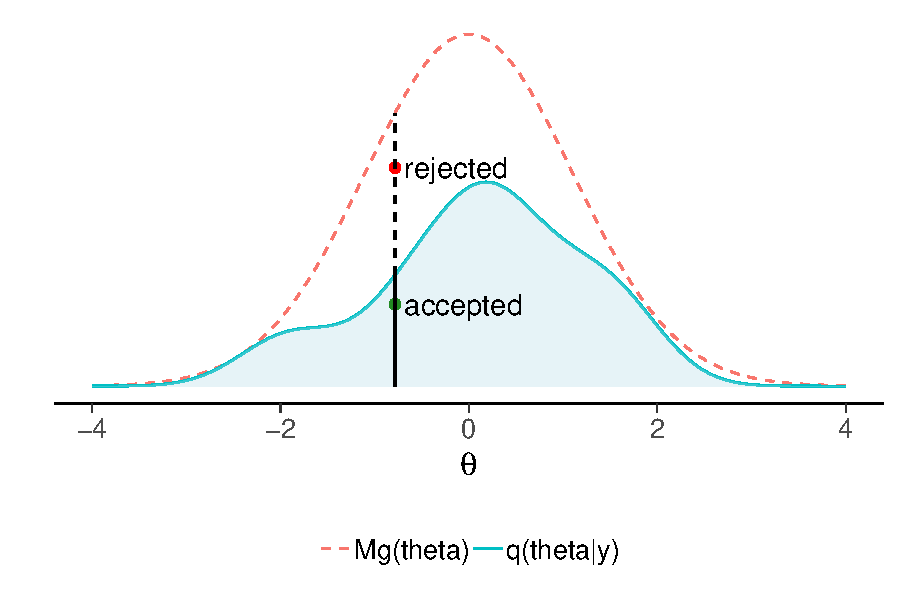
\includegraphics[width=10cm]{rejection1.pdf}}
    \only<2>{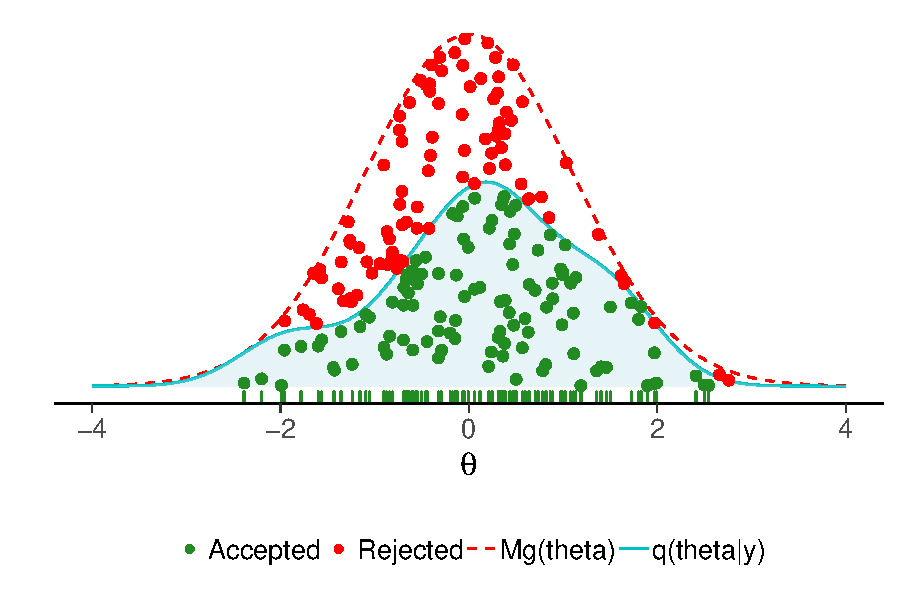
\includegraphics[width=10cm]{rejection2.pdf}}
    \only<3>{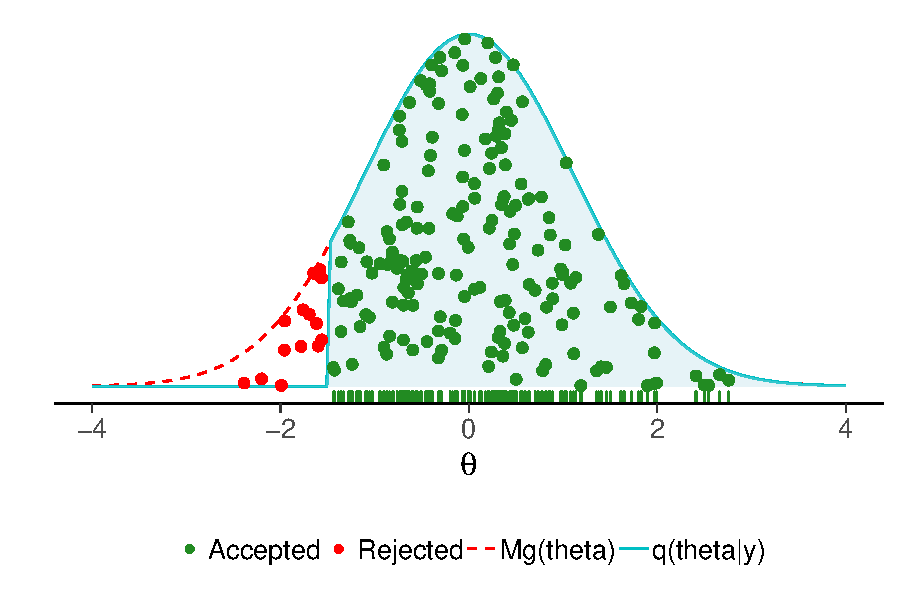
\includegraphics[width=10cm]{rejection3.pdf}}
  \end{center}

\end{frame}

\begin{frame}
  
  {\Large\color{navyblue} Rejection sampling}

  \begin{itemize}
  \item The number of accepted samples is the effective sample size
    \begin{itemize}
    \item with bad proposal distribution may require a lot of trials
    \item selection of good proposal gets very difficult when
      the number of dimensions increase
    \item reliable diagnostics and thus can be a useful part
    \end{itemize}
  \end{itemize}

\end{frame}


\begin{frame}
  
  {\Large\color{navyblue} Importance sampling}

  \begin{itemize}
     \vspace{-.5\baselineskip}
   \item[-] Proposal does not need to have a higher value everywhere
   \end{itemize}
   \begin{center}
     \vspace{-1\baselineskip}
     \only<1-2>{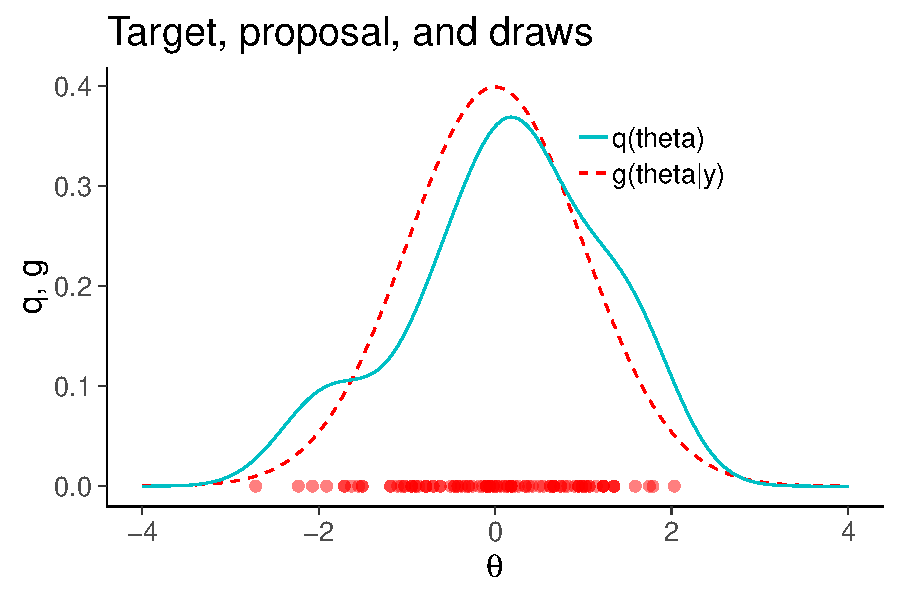
\includegraphics[width=9cm]{importancesamp1.pdf}}
     \only<3>{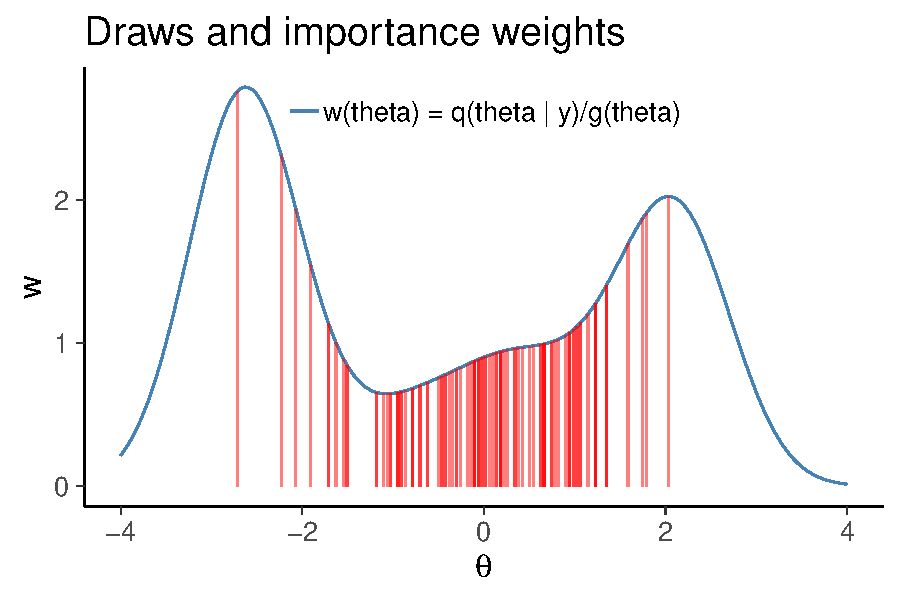
\includegraphics[width=9cm]{importancesamp2.pdf}}
     \vspace{-1\baselineskip}
     \only<2->{
   \begin{eqnarray*}
      \E[f(\theta)] \approx \frac{\sum_s w_s f(\theta^{(s)})}{\sum_s
      w_s}, \qquad \text{where} \quad 
      w_s =  \frac{q(\theta^{(s)})}{g(\theta^{(s)})} \qquad
   \end{eqnarray*}
   }
   \end{center}

\end{frame}

\begin{frame}
  
  {\Large\color{navyblue} Importance sampling}

  \begin{itemize}
  \item Resampling using normalized importance weights can be used to
    pick a smaller number of draws with uniform weights
  \item Selection of good proposal gets more difficult when the
      number of dimensions increase
    \item Often used to correct distributional approximations
  \end{itemize}

\end{frame}

\begin{frame}
  
  {\Large\color{navyblue} Importance sampling}

  \begin{itemize}
  \item Variation of the weights affect the effective sample size
    \begin{itemize}
    \item if single weight dominates, we have effectively one sample
    \item if weights are equal, we have effectively $S$ samples
    \end{itemize}
  \item Central limit theorem holds only if variance of the weight
    distribution is finite
  \item See Vehtari, Gelman and Gabry (2017). Pareto smoothed
    importance sampling. arXiv preprint arXiv:1507.02646,
    \url{https://arxiv.org/abs/1507.02646} for improved diagnostics
    and stability.
  \end{itemize}

\end{frame}

\begin{frame}
  
  {\Large\color{navyblue} Exmple: Importance sampling in Bioassay}

   \vspace{-.5\baselineskip}
   \makebox[12cm][t]{
     \hspace{-0.9cm}
     \begin{minipage}[t][12cm][t]{12cm}
       \begin{center}
        \makebox[0cm][t]{\hspace{-0.5cm}\rotatebox{90}{\hspace{1cm}Grid}}
        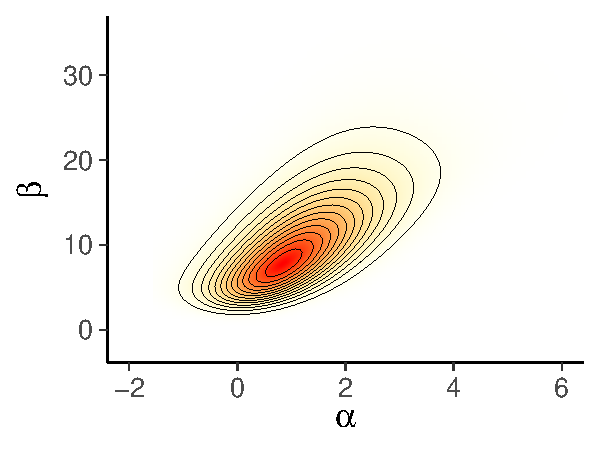
\includegraphics[width=3.4cm]{bioassayis1d.pdf}
      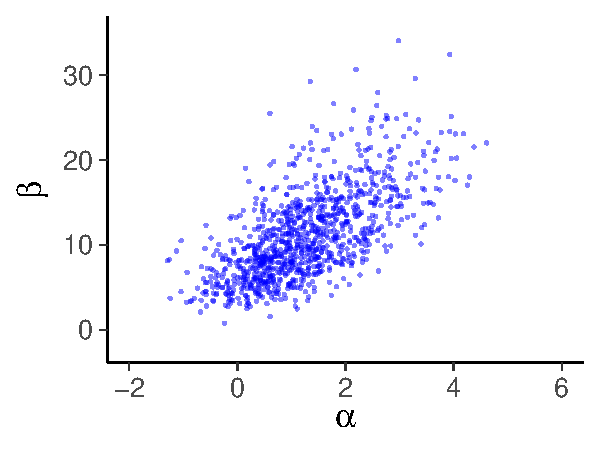
\includegraphics[width=3.4cm]{bioassayis1s.pdf}
      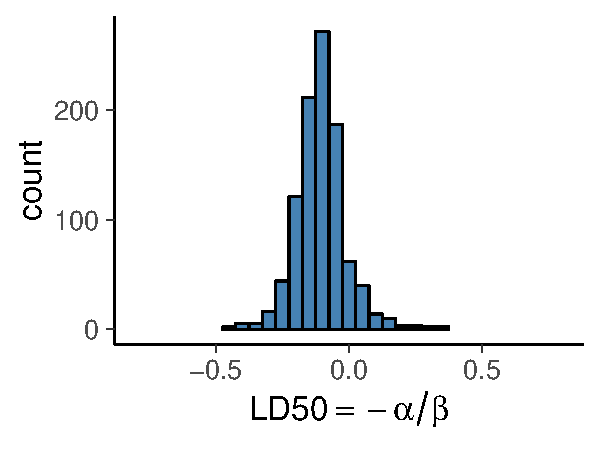
\includegraphics[width=3.4cm]{bioassayis1h.pdf}\\
      \only<2->{
        \makebox[0cm][t]{\hspace{-0.5cm}\rotatebox{90}{\hspace{1cm}Normal}}
      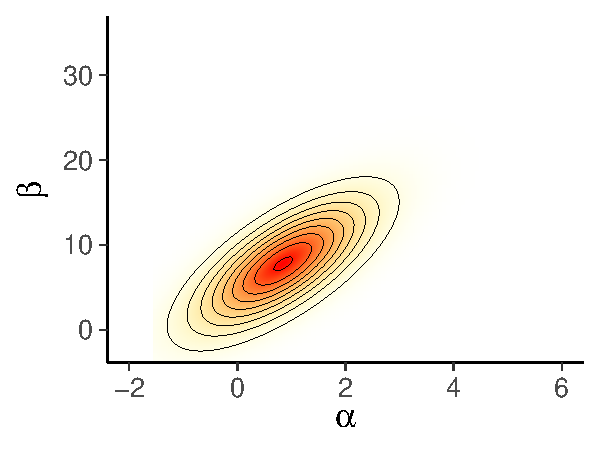
\includegraphics[width=3.4cm]{bioassayis2d.pdf}
      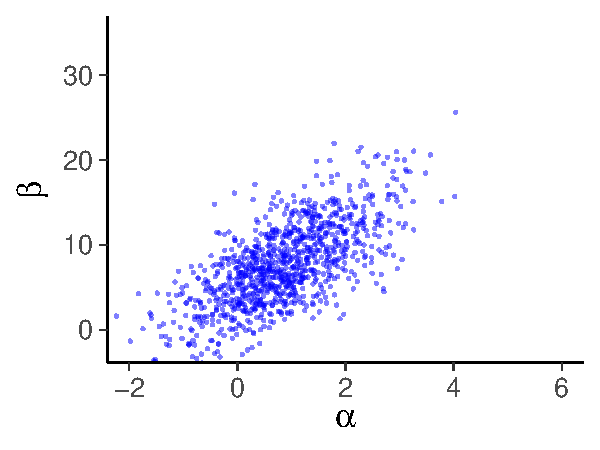
\includegraphics[width=3.4cm]{bioassayis2s.pdf}
      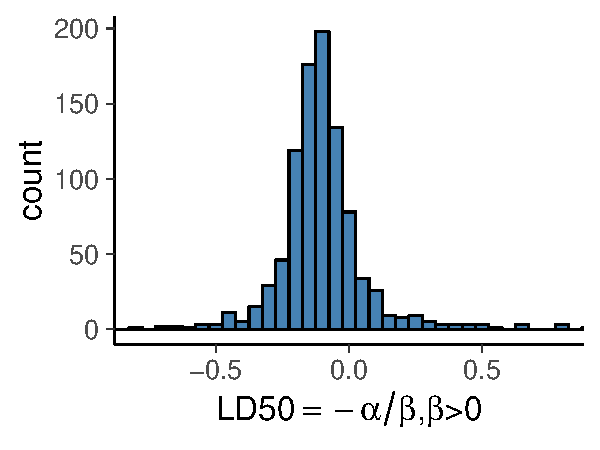
\includegraphics[width=3.4cm]{bioassayis2h.pdf}\\}
    \only<2-3>{Normal approximation is discussed more in BDA3 Ch 4\\}
    \only<3>{But the normal approximation is not that good here:\\ Grid sd(LD50) $\approx$ 0.1, Normal sd(LD50) $\approx$ .75!}
      \only<4->{
        \makebox[0cm][t]{\hspace{-0.5cm}\rotatebox{90}{\hspace{1cm}SIR}}
      
\includegraphics[width=3.4cm]{bioassayis3d.pdf}
      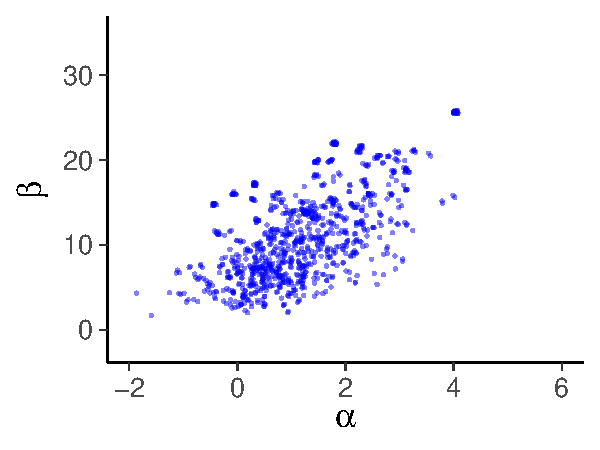
\includegraphics[width=3.4cm]{bioassayis3s.pdf}
      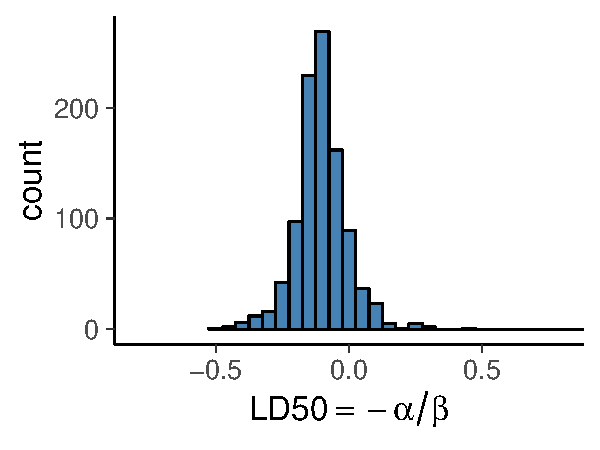
\includegraphics[width=3.4cm]{bioassayis3h.pdf}\\}
    \only<5->{Grid sd(LD50) $\approx$ 0.1, SIR sd(LD50) $\approx$ 0.1}
    \end{center}
     \end{minipage}  
   }
  
\end{frame}

\begin{frame}
  
  {\Large\color{navyblue} Exmple: Importance sampling in Bioassay}


   \makebox[12cm][t]{
     \hspace{-0.9cm}
     \begin{minipage}[t][6cm][t]{6cm}
       \begin{center}
       Grid\\
       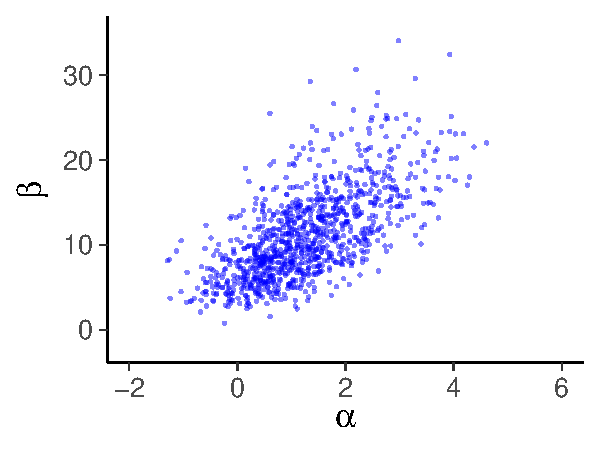
\includegraphics[width=6cm]{bioassayis1s.pdf}
     \end{center}
     \end{minipage}
     \begin{minipage}[t][6cm][t]{6cm}
       \begin{center}
       SIR\\
       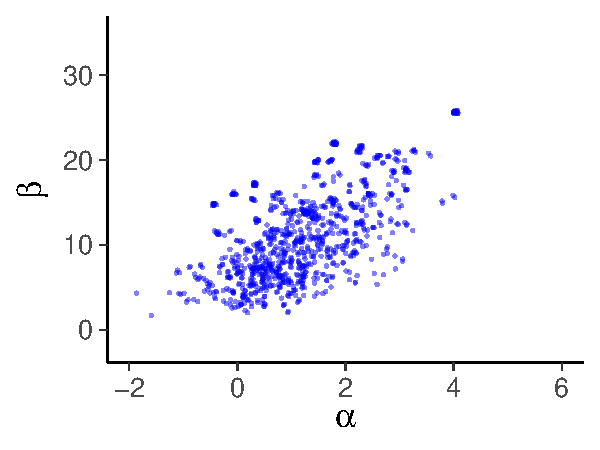
\includegraphics[width=6cm]{bioassayis3s.pdf}
  \end{center}
  \end{minipage}
}

\end{frame}

\begin{frame}
  
  {\Large\color{navyblue} Exmple: Importance sampling in Bioassay}

       \begin{center}
       SIR\\
       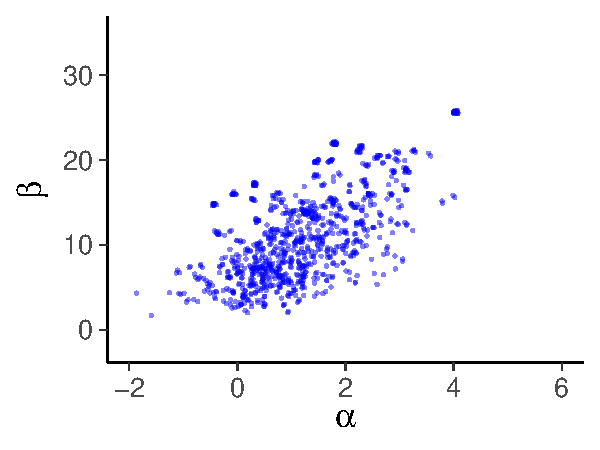
\includegraphics[width=10cm]{bioassayis3s.pdf}
  \end{center}

\end{frame}

\begin{frame}
  
  {\Large\color{navyblue} Exmple: Importance sampling in Bioassay}

       \begin{center}
       \only<1>{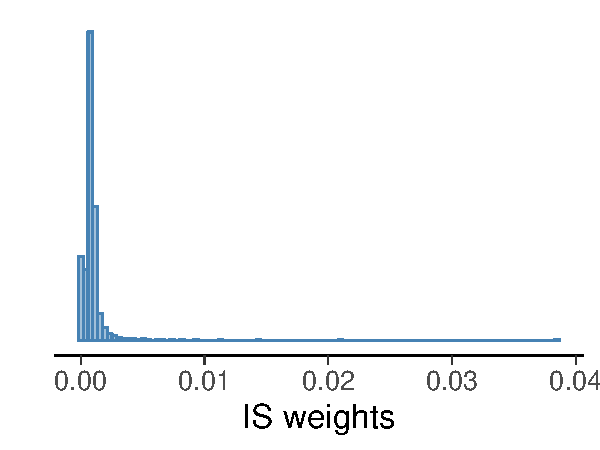
\includegraphics[width=10cm]{bioassayisw1.pdf}}
       \only<2>{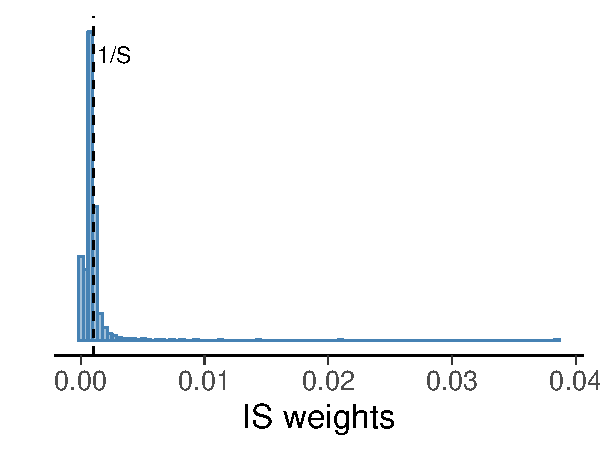
\includegraphics[width=10cm]{bioassayisw2.pdf}}
       \only<3>{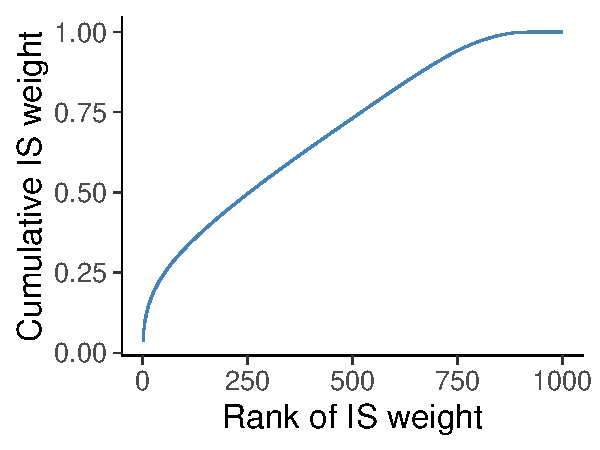
\includegraphics[width=10cm]{bioassayisw3.pdf}}
  \end{center}

\end{frame}

\begin{frame}
  
  {\Large\color{navyblue} Exmple: Importance sampling in Bioassay}

       \begin{center}
         \vspace{-\baselineskip}
       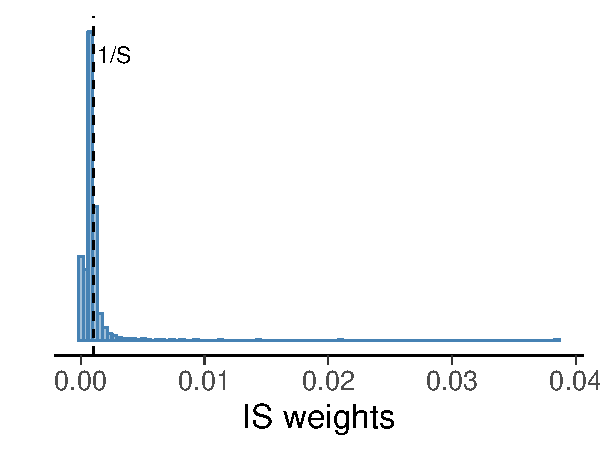
\includegraphics[width=8cm]{bioassayisw2.pdf}\\
         \vspace{-2\baselineskip}
         \begin{align*}
           S_{\rm eff} & = \frac{1}{\sum_{s=1}^S (\tilde{w}(\theta^s))^2}, \quad \text{where } \tilde{w}(\theta^s)=w(\theta^s)/\sum_{s'=1}^Sw(\theta^{s'})\\
           \uncover<2->{S_{\rm eff} & \approx 270}
         \end{align*}
  \end{center}

\end{frame}

\begin{frame}
  
  {\Large\color{navyblue} Exmple: Importance sampling in Bioassay}

       \begin{center}
         \vspace{-\baselineskip}
       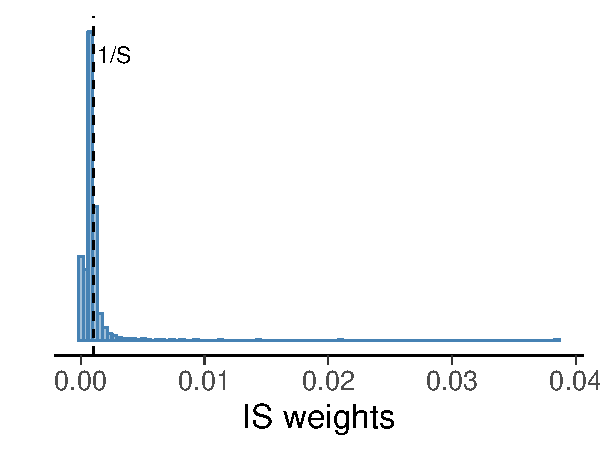
\includegraphics[width=8cm]{bioassayisw2.pdf}\\
         \vspace{-2\baselineskip}
         \begin{align*}
           S_{\rm eff} & = \frac{1}{\sum_{s=1}^S (\tilde{w}(\theta^s))^2}, \quad \text{is based on variance of } \tilde{w}(\theta^s) \\
           S_{\rm eff} & \approx 270 \\ \uncover<2->{&\text{Pareto-$k$ diagnostic preferably < 0.7: }}\uncover<3->{ \hat{k} \approx 0.76}
         \end{align*}
  \end{center}

\end{frame}

\begin{frame}
  
  {\Large\color{navyblue} Pareto smoothed importance sampling}


  \begin{itemize}
  \item Pareto-$k$ diagnostic estimate the number of existing moments ($\lfloor 1/k \rfloor$)
  \item Finite variance and central limit theorem for $k<1/2$
  \item Finite mean and generalized central limit theorem for $k<1$,
    but pre-asymptotic constant grows impractically large for $k>0.7$
  \item See Vehtari, Gelman and Gabry (2017). Pareto smoothed
    importance sampling. arXiv preprint arXiv:1507.02646,
    \url{https://arxiv.org/abs/1507.02646} for improved diagnostics
    and stability.
  \end{itemize}
\end{frame}

\begin{frame}
  
  {\Large\color{navyblue} Importance sampling leave-one-out cross-validation}

  \begin{itemize}
  \item Later in the course you will learn how $p(\theta|y)$ can be
    used as a proposal distribution for $p(\theta|y_{-i})$
    \begin{itemize}
    \item which allows fast computation of leave-one-out cross-validation
      \begin{align*}
        p(y_i|y_{-i})=\int p(y_i|\theta) p(\theta|y_{-i}) d\theta
      \end{align*}
    \end{itemize}
  \end{itemize}

\end{frame}

\begin{frame}
  
  {\Large\color{navyblue} Curse of dimensionality}

  \begin{itemize}
  \item Number of grid points increases exponentially
  \item Concentration of the measure, ie, where is the most of the
    mass?
  \end{itemize}

\end{frame}

\begin{frame}
  
  {\Large\color{navyblue} Markov chain Monte Carlo (MCMC)}

  \begin{itemize}
  \item Markov chain goes where most of the posterior mass is
  \item Certain MCMC methods scale well to high dimensions
  \item MCMC methods in this course
    \begin{itemize}
    \item Gibbs: ``iterative conditional sampling''
    \item Metropolis: ``random walk in joint distribution''
    \item Dynamic Hamiltonian Monte Carlo: ``state-of-the-art'' used in Stan
    \end{itemize}
  \end{itemize}

\end{frame}

\end{document}

%%% Local Variables: 
%%% TeX-PDF-mode: t
%%% TeX-master: t
%%% End: 
